%% \documentclass[landscape,final,a0paper,fontscale=0.285]{baposter}
\documentclass[landscape,final,a0paper,fontscale=0.32]{baposter}
%% \documentclass[landscape,final,a0paper,fontscale=0.4]{baposter}
%% \documentclass[landscape,final,a0paper,fontscale=0.35]{baposter}

\usepackage{calc}
\usepackage{graphicx}
\usepackage{amsmath}
\usepackage{amssymb}
\usepackage{relsize}
\usepackage{multirow}
\usepackage{rotating}
\usepackage{bm}
\usepackage{url}

\usepackage{graphicx}
\usepackage{multicol}

%% \usepackage{times}
%% \usepackage{helvet}
%\usepackage{bookman}
\usepackage{palatino}

\usepackage{lipsum}
%% \usepackage{jabbrv}
%% \usepackage{setspace}
\usepackage{enumitem}

\newcommand{\captionfont}{\footnotesize}

\graphicspath{{../paper/figures/}}
%% \graphicspath{{images/}{../images/}}
%% \usetikzlibrary{calc}

%%%%%%%%%%%%%%%%%%%%%%%%%%%%%%%%%%%%%%%%%%%%%%%%%%%%%%%%%%%%%%%%%%%%%%%%%%%%%%%%
%%%% Some math symbols used in the text
%%%%%%%%%%%%%%%%%%%%%%%%%%%%%%%%%%%%%%%%%%%%%%%%%%%%%%%%%%%%%%%%%%%%%%%%%%%%%%%%

%%%%%%%%%%%%%%%%%%%%%%%%%%%%%%%%%%%%%%%%%%%%%%%%%%%%%%%%%%%%%%%%%%%%%%%%%%%%%%%%
% Multicol Settings
%%%%%%%%%%%%%%%%%%%%%%%%%%%%%%%%%%%%%%%%%%%%%%%%%%%%%%%%%%%%%%%%%%%%%%%%%%%%%%%%
\setlength{\columnsep}{1.5em}
\setlength{\columnseprule}{0mm}

%%%%%%%%%%%%%%%%%%%%%%%%%%%%%%%%%%%%%%%%%%%%%%%%%%%%%%%%%%%%%%%%%%%%%%%%%%%%%%%%
% Save space in lists. Use this after the opening of the list
%%%%%%%%%%%%%%%%%%%%%%%%%%%%%%%%%%%%%%%%%%%%%%%%%%%%%%%%%%%%%%%%%%%%%%%%%%%%%%%%
\newcommand{\compresslist}{%
\setlength{\itemsep}{1pt}%
\setlength{\parskip}{0pt}%
\setlength{\parsep}{0pt}%
}

%%%%%%%%%%%%%%%%%%%%%%%%%%%%%%%%%%%%%%%%%%%%%%%%%%%%%%%%%%%%%%%%%%%%%%%%%%%%%%
%%% Begin of Document
%%%%%%%%%%%%%%%%%%%%%%%%%%%%%%%%%%%%%%%%%%%%%%%%%%%%%%%%%%%%%%%%%%%%%%%%%%%%%%

\begin{document}

%%%%%%%%%%%%%%%%%%%%%%%%%%%%%%%%%%%%%%%%%%%%%%%%%%%%%%%%%%%%%%%%%%%%%%%%%%%%%%
%%% Here starts the poster
%%%---------------------------------------------------------------------------
%%% Format it to your taste with the options
%%%%%%%%%%%%%%%%%%%%%%%%%%%%%%%%%%%%%%%%%%%%%%%%%%%%%%%%%%%%%%%%%%%%%%%%%%%%%%
% Define some colors

%\definecolor{lightblue}{cmyk}{0.83,0.24,0,0.12}
%% \definecolor{lightblue}{rgb}{0.145,0.6666,1}

%% \definecolor{headerfade}{rgb}{0.89,0.68,0}
\definecolor{headerfade}{rgb}{0.93, 0.80, 0.38}

\hyphenation{resolution occlusions}
%%
\begin{poster}%
  % Poster Options
  {
  % Show grid to help with alignment
  grid=false,
  columns=4,
  % Column spacing
  colspacing=1em,
  % Color style
  bgColorOne=white,
  bgColorTwo=white,
  borderColor=headerfade,
  headerColorOne=black,
  headerColorTwo=headerfade,
  headerFontColor=white,
  boxColorOne=white,
  boxColorTwo=headerfade,
  % Format of textbox
  textborder=roundedleft,
  % Format of text header
  eyecatcher=true,
  headerborder=closed,
  headerheight=0.17\textheight,
%  textfont=\sc, An example of changing the text font
  headershape=roundedright,
  headershade=shadelr,
  headerfont=\Large\bf\textsc, %Sans Serif
  textfont={\setlength{\parindent}{1.5em}},
  boxshade=plain,
%  background=shade-tb,
  background=plain,
  linewidth=2pt
  }
  % Eye Catcher
  {
    \begin{tabular}{c}
      \relax\\
      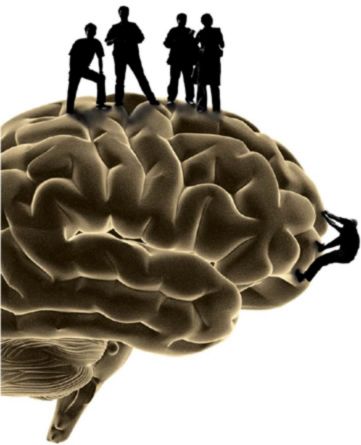
\includegraphics[height=13em]{brain.png}
    \end{tabular}
  }
  % Title
  {
    \textbf{\textsc{Selective Processing for\\[0.2em] Real-time Stereo Matching}}\vspace{0.5em}
  }
  % Authors
  {
    \textsc{Eric Hunsberger, Jeff Orchard, Bryan Tripp}\\[0.2em]
    \{ehunsber, jeff.orchard, bptripp\}@uwaterloo.ca\\[0.4em]
    %% Centre for Theoretical Neuroscience, University of Waterloo (\url{http://ctn.uwaterloo.ca})
  }
  % University logo
  {
    %% 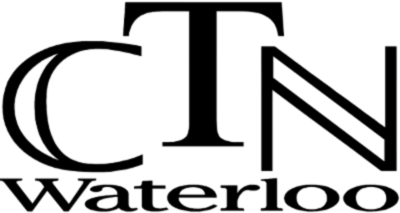
\includegraphics[height=9.0em]{ctn.png}
    \begin{tabular}{cc}
      \relax\\
      
\includegraphics[height=6.0em]{uwaterloo.png} &
      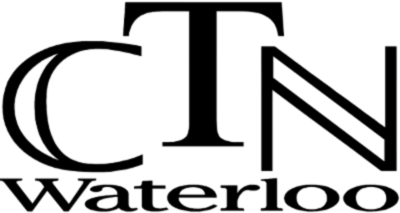
\includegraphics[height=5.0em]{ctn.png}\\
      \multicolumn{2}{c}{
        
\includegraphics[height=5.0em]{cnrg.png}}
    \end{tabular}
  }

%%%%%%%%%%%%%%%%%%%%%%%%%%%%%%%%%%%%%%%%%%%%%%%%%%%%%%%%%%%%%%%%%%%%%%%%%%%%%%
%%% Now define the boxes that make up the poster
%%%---------------------------------------------------------------------------
%%% Each box has a name and can be placed absolutely or relatively.
%%% The only inconvenience is that you can only specify a relative position
%%% towards an already declared box. So if you have a box attached to the
%%% bottom, one to the top and a third one which should be in between, you
%%% have to specify the top and bottom boxes before you specify the middle
%%% box.
%%%%%%%%%%%%%%%%%%%%%%%%%%%%%%%%%%%%%%%%%%%%%%%%%%%%%%%%%%%%%%%%%%%%%%%%%%%%%%
    %
    % A coloured circle useful as a bullet with an adjustably strong filling
    \newcommand{\colouredcircle}{%
      \tikz{\useasboundingbox (-0.2em,-0.32em) rectangle(0.2em,0.32em); \draw[draw=black,fill=headerfade,line width=0.03em] (0,0) circle(0.18em);}}

    \newenvironment{blockitemize}
    {%
      \noindent\hspace{-1em}
      \begin{minipage}{\columnwidth}
      \begin{itemize}
        \setlength{\itemsep}{0.3em}

        \raggedright
    }{
      \end{itemize}
      \end{minipage}
    }

    %%%%%%%%%%%%%%%%%%%%%%%%%%%%%%%%%%%%%%%%%%%%%%%%%%%%%%%%%%%%%%%%%%%%%%%%%%%%%%%%

    \headerbox{Introduction}{name=pane00,column=0,row=0}{
      \begin{blockitemize}
        \item Multiscale Belief Propagation (BP) is an accurate
          stereo-matching algorithm.
        \item Our goal is to reduce computation time while maintaining accuracy
          by focusing computation in important regions of the image. We will
          call the important region in a particular frame the \emph{fovea},
          analogous to the fovea of the eye.
        \item We also want to incorporate past data into the depth estimate
          for the current frame.
      \end{blockitemize}
    }

    \headerbox{Belief Propagation}{name=pane01,column=0,below=pane00}{
      \begin{center}
        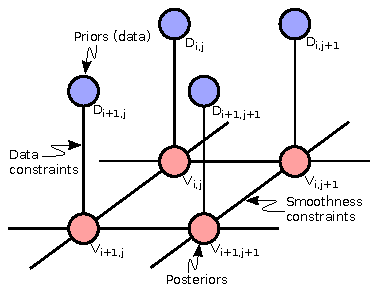
\includegraphics[width=0.7\columnwidth]{mrf.pdf}
        \vspace{-1em}
      \end{center}
      \noindent
      Belief Propagation (BP) \cite{Sun2003a} poses the stereo-matching problem in terms of
      the solution to a Markov Random Field. The ``loopy'' BP algorithm then
      uses a message-passing scheme to perform approximate inference on this
      field, resulting in probabilities across all possible disparity matches
      of all the pixels in the scene.

      Multiscale BP reduces the number of iterations
      by performing BP at a coarser resolution first,
      and using this to seed BP at a finer resolution \cite{Felzenszwalb2006a}.
      Iterations at the finest resolution take the most time.
      We reduce computation time by only treating part of the image at the
      finest scale, and using coarse results elsewhere.
    }

    \headerbox{References}{name=pane02,column=0,below=pane01,above=bottom}{
      \scriptsize
      \renewcommand{\refname}{\vspace{-0.8em}}
      \bibliographystyle{ieeetr}
      %% \bibliographystyle{jabbrv_ieeetr}
      \bibliography{../paper/fast-stereo-eric}
    }

    \headerbox{Fovea Example}{name=pane10,column=1,row=0}{
      \begin{center}
        %% 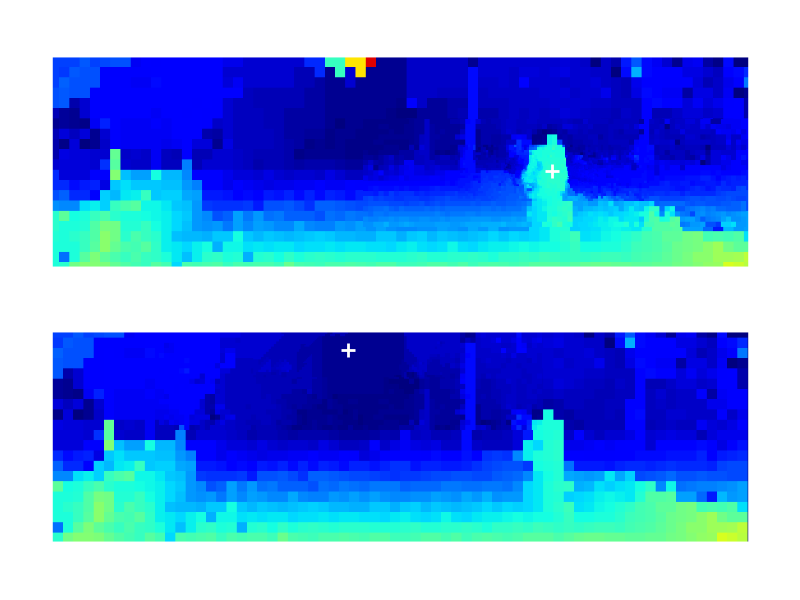
\includegraphics[width=0.75\columnwidth,clip=true,trim=50px 55px 50px 55px]{fovea-examples.png}
        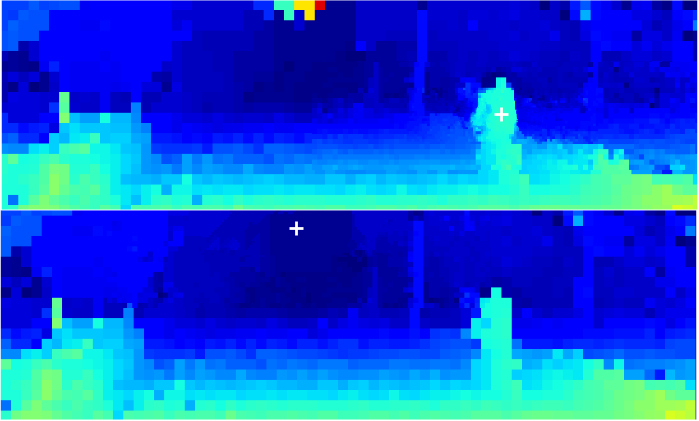
\includegraphics[width=0.9\columnwidth]{fovea-examples-tight.png}
      \end{center}
      The fovea can decrease error around important objects
      and help remove artifacts.
      In the top panel, the fovea is centred on the cyclist, a salient object.
      The coarse BP estimate has discovered a potential obstacle in the top of the frame.
      In the second frame, the fovea centres on this potential obstacle
      and discovers it was an artifact in the previous coarse BP computation;
      there is actually nothing there.
    }

    \headerbox{Coarse vs Fine BP}{name=pane11,column=1,row=0,below=pane10,above=bottom}{
      \begin{center}
        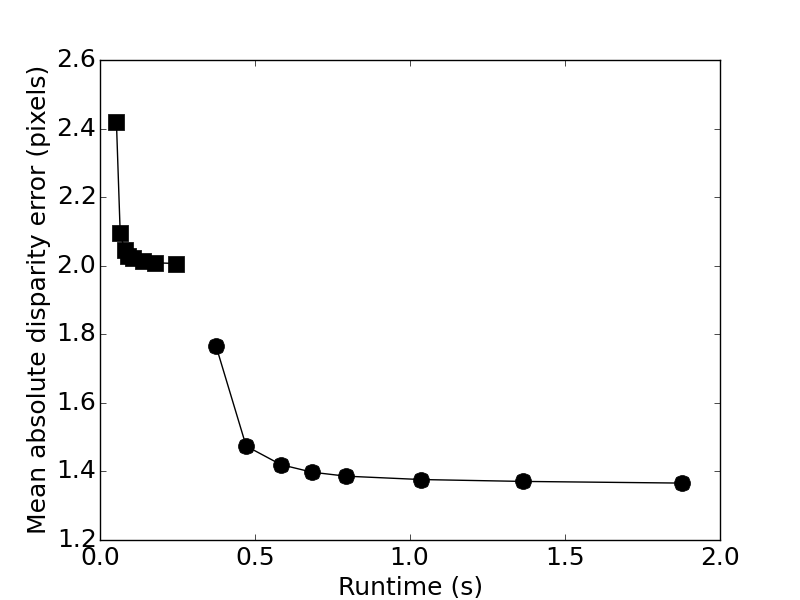
\includegraphics[width=1.0\columnwidth]{fovea-rationale.png}
      \end{center}
      Comparing runtime and error of BP at coarse (squares) and fine (circles)
      resolutions across different numbers of iterations,
      we see that using more iterations to coarse BP quickly saturates in performance,
      whereas adding iterations to fine BP quickly makes the runtime too long for real time.
      By applying fine BP selectively to important regions,
      we can achieve real-time BP (at 10 Hz) with better performance than coarse BP.
    }

    %% \headerbox{Importance}{name=pane20,column=2,row=0}{
    %%   \begin{center}
    %%     %% 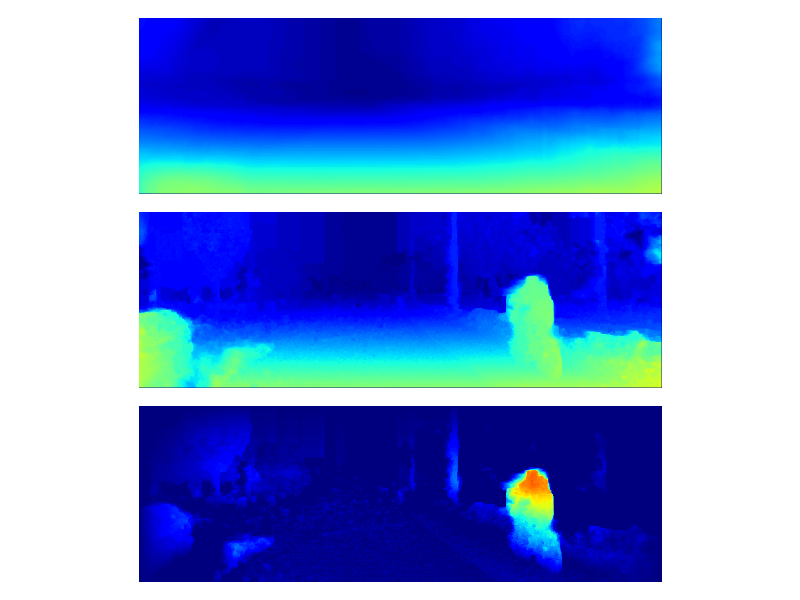
\includegraphics[width=1.0\columnwidth]{importance.png}
    %%     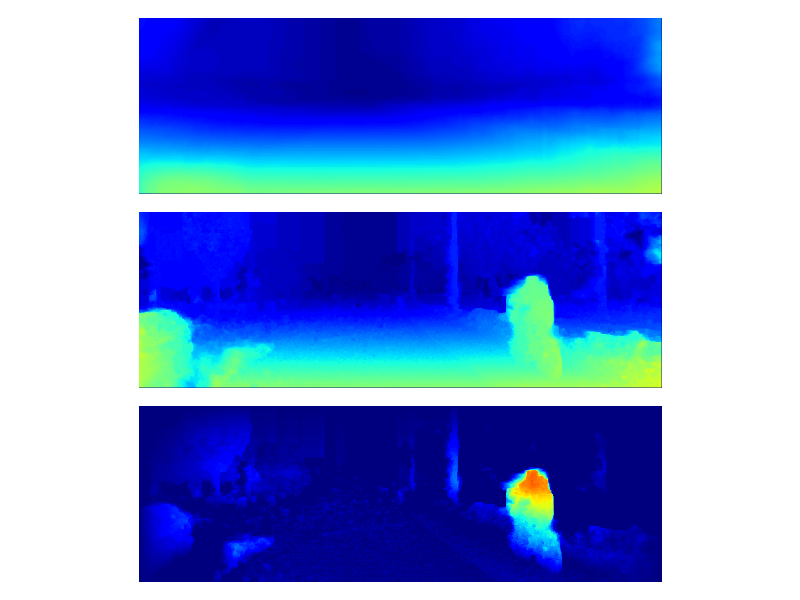
\includegraphics[width=0.6\columnwidth,clip=true,trim=130px 15px 130px 15px]{importance.png}
    %%   \end{center}
    %%   To choose regions of interest for foveation,
    %%   we compare the current coarse depth estimate (middle)
    %%   with the average depth estimate across many frames (top).
    %%   The difference highlights regions that are unexpectedly close (bottom).
    %% }

    %% \headerbox{Foveation sequence}{name=pane21,column=2,row=0,below=pane20}{
    %%   TODO
    %%   \begin{center}
    %%     %% 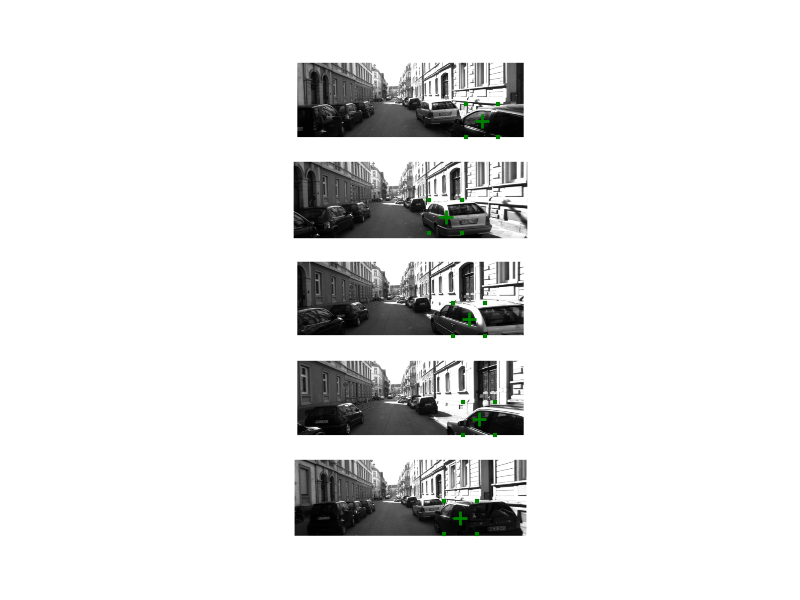
\includegraphics[width=1.0\columnwidth,clip=true,trim=220px 100px 200px 120px]{foveation-sequence.png}
    %%     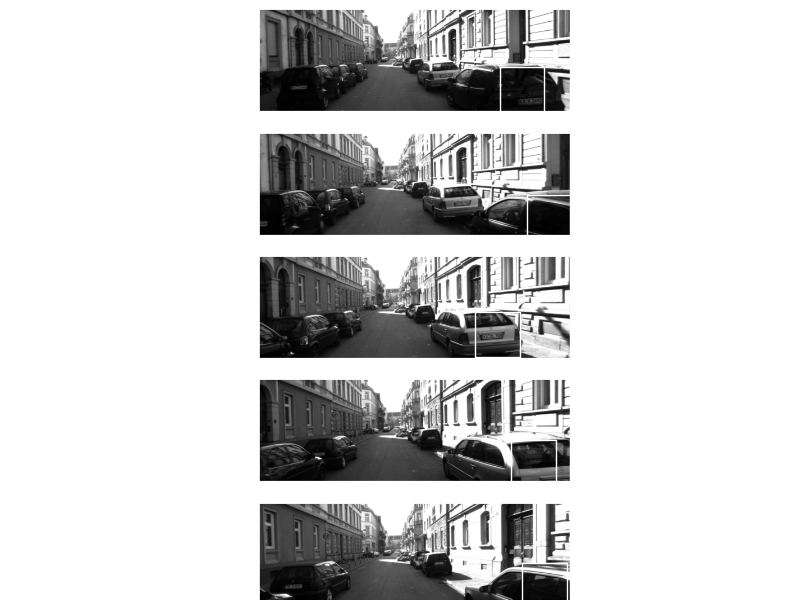
\includegraphics[width=0.6\columnwidth]{foveation-sequence-tight.png}
    %%   \end{center}
    %% }

    \headerbox{Choosing Fovea Locations}{name=pane20,column=2,row=0}{
      %% \begin{minipage}
      %% \begin{multicols}{2}
      %% \end{multicols}
      %% \end{minipage}

      %% \begin{center}
      %%   %% 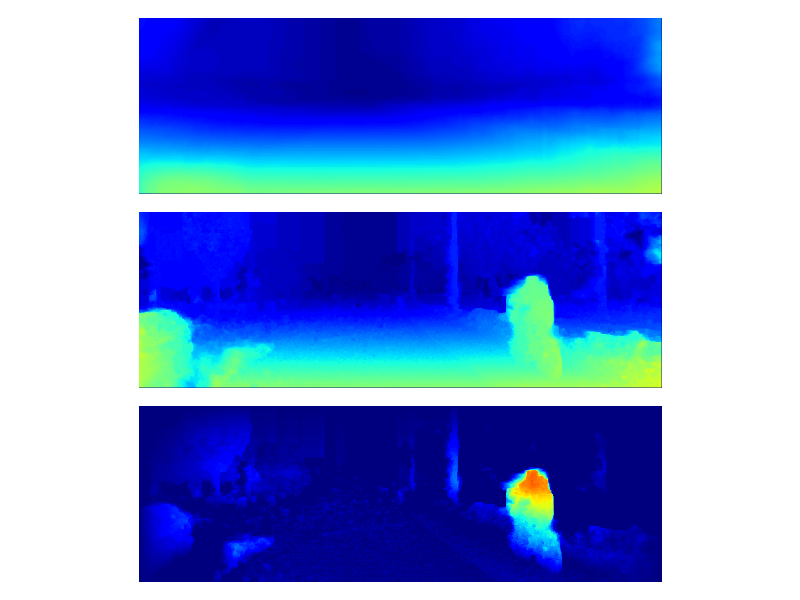
\includegraphics[width=1.0\columnwidth]{importance.png}
      %%   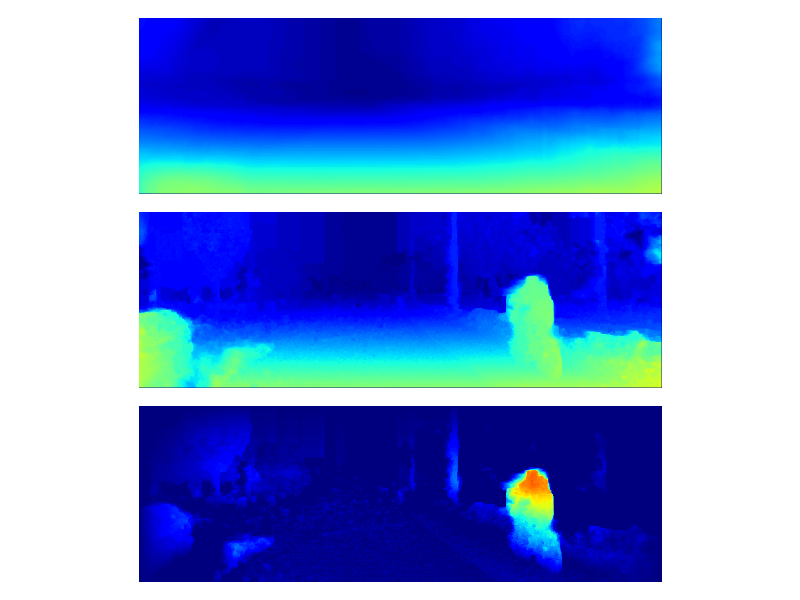
\includegraphics[width=0.6\columnwidth,clip=true,trim=130px 15px 130px 15px]{importance.png}
      %% \end{center}

      \begin{center}
      \begin{tabular}{ll}
        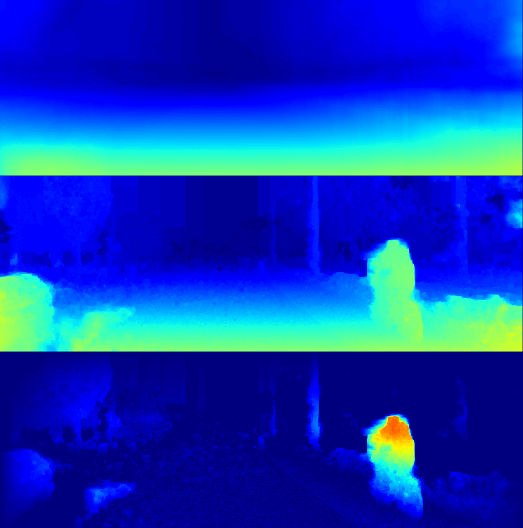
\includegraphics[width=0.6\columnwidth]{importance-tight.png} &
        \hspace{-1em}
        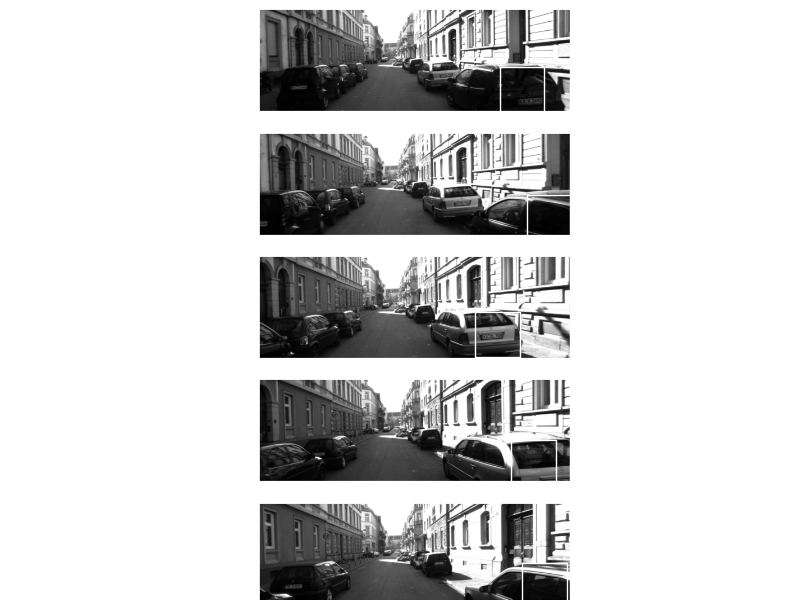
\includegraphics[width=0.37\columnwidth]{foveation-sequence-tight.png}
      \end{tabular}
      \end{center}

      \noindent
      To choose regions of interest for foveation,
      we designed a simple metric for assigning importance $I$ to pixels:
      \begin{equation}
        I = \max(V_{coarse} - V_{average}, 0)
        \label{eqn:importance}
      \end{equation}
      Regions where the coarse depth estimate $V_{coarse}$ (left middle)
      is closer than the average depth $V_{average}$ (left top)
      are where a collision is most likely (left bottom).
      %% we compare the current coarse depth estimate (left middle)
      %% with the average depth estimate across many frames (left top).
      %% The difference highlights regions that are unexpectedly close (left bottom).

      The right shows an example foveation sequence computed using this algorithm.
      The fovea follows the nearby obstacles, since these are the most different
      from the expected depth and the highest risk of collision.
    }

    \headerbox{Filtering Over Time}{name=pane21,column=2,row=0,below=pane20,above=bottom}{
      \begin{center}
        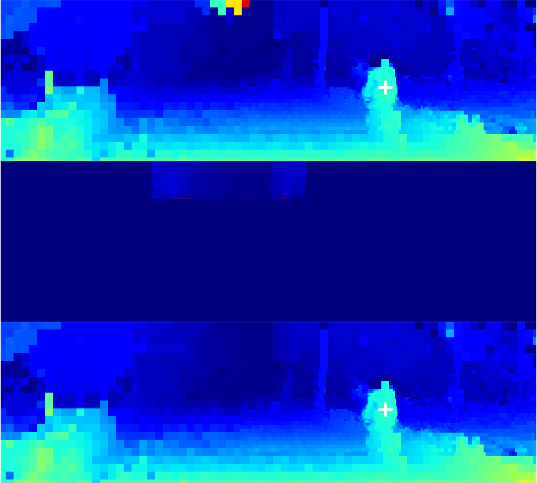
\includegraphics[width=0.6\columnwidth]{seed-vs-no-seed-tight.png}
      \end{center}
      Remembering information from previous fovea locations can further improve results.
      In the top frame, we see an artifact (error) in the coarse BP solution.
      Using information from a previous foveation to that location (centre),
      the artifact can be removed by using the past information as a seed
      for BP (bottom).
    }

    \headerbox{Results}{name=pane30,column=3,row=0}{
      \noindent
      We tested our algorithm on the KITTI dataset stereo evaluation dataset
      \cite{Geiger2012CVPR}.
      This dataset is composed of driving sequences recorded
      with ground-truth depth information from a LIDAR scanner.
      We computed errors on both the raw LIDAR points,
      and a weighted-average version prioritizing points with high
      importance (see Equation~\ref{eqn:importance}).

      \vspace{1em}
      \begin{tabular}{|l|r|r|r|}
        \hline
        & Unweighted & Weighted & Time \\\hline
        Coarse & 2.413 px & 5.115 px & 0.06 s \\
        Fine & 1.890 px & 4.241 px & 0.47 s \\

        % --- results using fine data cost
        \textbf{Fovea} & \textbf{1.904 px} & \textbf{4.380 px} & \textbf{0.16 s}\\\hline
        %% \textbf{Fovea (coarse cost)} & \textbf{1.904 px} & \textbf{4.380 px} & \textbf{0.15 s}\\\hline

        % --- results using coarse data cost

      \end{tabular}
      \vspace{1em}

      The results show that the foveal method has error levels close to
      that of fine-scale BP,
      while the computation time is much closer to coarse BP.
      The computation time is not quite real-time (10 Hz),
      though currently we are computing disparities for the top part
      of the image which is not tested by the LIDAR points;
      removing this should result in real-time computation.
    }

    \headerbox{Conclusions}{name=pane31,column=3,row=0,below=pane30}{
      \begin{blockitemize}
        \item Focusing computation on specific regions of the image
          achieves a balance between fast computation time and low error.
        \item A simple importance metric (Equation~\ref{eqn:importance})
          directs computational resources to where they are most needed
          for vehicle navigation.
        \item Tracking information over time removes artifacts
          that tend to appear in only one frame in a sequence.

        %% \item Computing the data cost at higher
        %% \item Computing the fine data cost and downsampling has
      \end{blockitemize}
    }

    \headerbox{Future Work}{name=pane32,column=3,row=0,below=pane31,above=bottom}{
      \begin{blockitemize}
        \item Determine what portion of the results are due to the fovea position,
          and what portion are because the foveal method uses the fine data cost.
        \item Use coarser resolution outside the fovea to further reduce computation.
        \item Use multiple foveas to target multiple regions of interest.
        \item Use point tracking to better accommodate noisy GPS data
          and object motion when integrating information over time.
      \end{blockitemize}
    }

\end{poster}
\end{document}

%%  LocalWords:  headerfade rgb colspacing bgColorOne bgColorTwo TODO
%%  LocalWords:  borderColor headerColorOne headerColorTwo textborder
%%  LocalWords:  headerFontColor boxColorOne boxColorTwo roundedleft
%%  LocalWords:  eyecatcher headerborder headerheight headershape px
%%  LocalWords:  roundedright headershade shadelr headerfont textfont
%%  LocalWords:  boxshade linewidth uwaterloo ehunsber
%%  LocalWords:  rasters multi Tripp jeff bptripp Multiscale
%%  LocalWords:  runtime foveation KITTI LIDAR Unweighted foveal GPS
